90. \begin{figure}[ht!]
\center{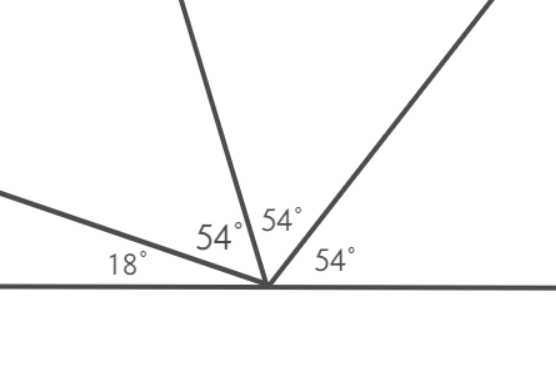
\includegraphics[scale=0.35]{g90.png}}
\end{figure}\\Проведём прямую и отложим из одной точки три угла, равных $54^\circ,$ как показано на рисунке. Тогда оставшийся угол равен $180^\circ-3\cdot54^\circ=18^\circ.$ Это как раз треть от $54^\circ,$ так что остаётся только построить два угла, равных полученному, внутри одного из углов, равных $54^\circ.$\\
